%===================================================
\section{Propagation et spécificités des sources aéroacoustiques}
%===================================================
On décrit ici les sources de bruit d'un avion à turbopropulseur, les méthodes de séparation des différentes contributions et les mécanismes de génération de bruits en écoulement.\\


Le bruit peut être généralement décomposé en 4 composantes : \\
-une partie tonale générée par les composantes tournantes de la machine\\
-une partie cyclostationnaire induite par les composantes tournantes de la machine\\
-le bruit machine aléatoire \\
-le bruit de fond (indépendant de la machine) (aérodynamique ?)\\


Séparer ces composantes dans le champ total mesuré permet de mieux comprendre la contribution de chaque source ou de chaque élément du réacteur, par exemple.



\subsection{Exemples de sources aéroacoustiques sur un avion}
%=============================================================

\todo[inline]{Un bref récap des sources est fait en intro de la thèse de Greboul}
\cite{smith} décrit un très grand nombre de sources aéroacoustisques sur un avion. Elles peuvent être classées en 2 catégories : le bruit de moteur et le bruit aérodynamique. Le bruit aérodynamique est principalement généré par le train d'atterrissage et par les ailes. La principale source de bruit des ailes est liée aux volets à l'avant (becs de bord d'attaque) et à l'arrière. Ces volets sont des hypersustentateurs qui augmentent la portance qui génèrent localement beaucoup de bruit. Mais paradoxalement, leur présence contribuent fortement à la réduction du bruit des avions par le fait qu'ils favorisent un décollage rapide et un atterrissage à vitesse réduite.\\
Comme le montre l'image de \cite{smith} \ref{smith}, les bruits du moteur sont d'origines diverses. Les moteurs doubles flux ont permis de fortement diminuer le bruit de jet, ce qui rend le bruit aérodynamique égal voire prépondérant sur le bruit de moteur en configuration d'approche (atterrissage).

\begin{figure}[!h]
 \begin{center}
  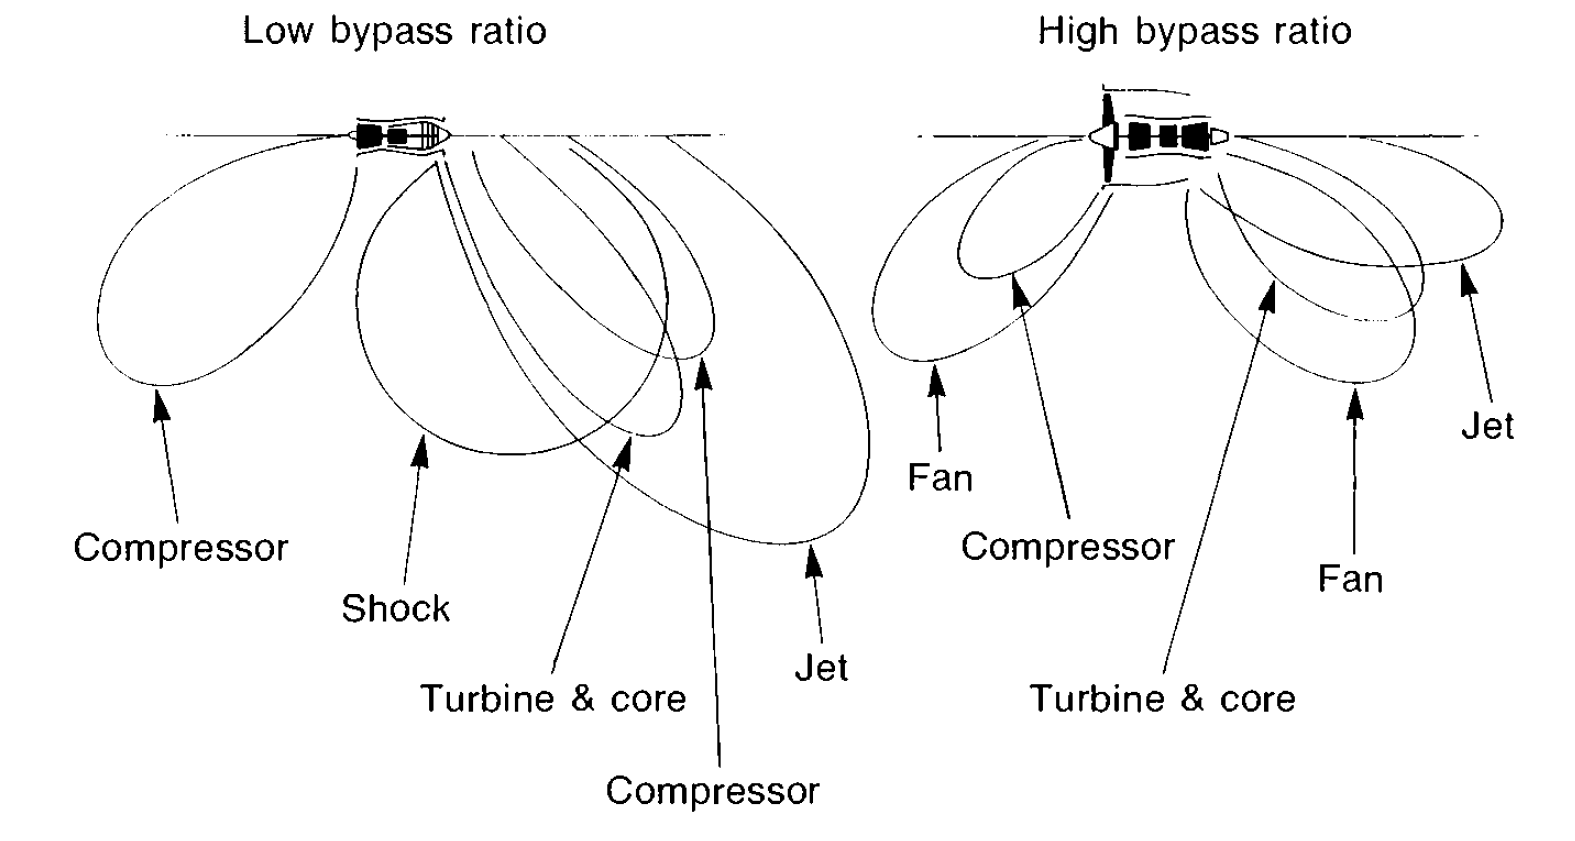
\includegraphics[width=0.5\textwidth]{img/smith_noise.png}
  \caption{Comparaison des sources de bruits d'un moteur simple flux (à gauche) et d'un moteur double flux (à droite). Image extraite de \cite{smith}.\label{smith}}
 \end{center}
\end{figure}

\subsubsection{Fan noise}

\paragraph{Bruits tonaux}
\begin{itemize}
	\item Fréquence de passage des pales (BPF : blade pass frequency) et ses harmoniques : bruit tonal, connu : $\omega = h Z \Omega$, $h=1,2,...$,  où $Z$ est le nombre de pales du rotor et $\Omega$ est sa fréquence de rotation. Les harmoniques qui apparaissent sont alors donnés par : $m=hZ-sV$, avec $m$ le numéro du mode azimutal, $V$ le nombre de pale du stator et $s=...,-1,0,1,...$\\
	\item Bruit d'épaisseur (Blade thickness noise) : monopole, tonal. C'est le bruit généré par le déplacement du fluide autour des pales (présent à haute vitesse de rotation seulement).\\
	\item Uniform inlet flow : peut être réduit en augmentant le nombre de pales\\
\end{itemize}
 

\paragraph{Bruits large bande}
\begin{itemize}
	\item Flux inconstant : fluctuation stochastique de la vitesse du flux entrant génère un bruit large bande\\
	\item Couche limite turbulente (TBL : Turbulent Boundary layer) : couche turbulent générée aux bords de fuite. Ce bruit peut être modélisé comme un ensemble de dipôles répartis sur la surface de l'aube.\\
	\item Décollement de couche limite (Vortex shedding) : décollement de la couche limite (laminaire ou turbulente), ce qui change l'écoulement autour des pales\\
	\item tip noise : bruit généré dans l'espacement entre les pales et le carter. Ce bruit augmente si l'espacement augmente. A noter que la vitesse à l'extrémité des pales étant grande, ce bruit peut être important.\\
	\item Bruit de soufflante : dans les turboréacteurs double-flux principalement. Ref : thèse Greboul\\
\end{itemize}

Bruit d'interaction rotor-stator : dominant ?

les moteur a double flux ont permis de diminuer l'importance du bruit de jet, mais a rajouté le bruit de soufflante.


\subsubsection{Bruit de jet}

page 86 de Smith : Description du bruit de jet\\
-small-scale Eddies (HF)\\
-large-scale Eddies (BF)\\
-mixing region\\
-shock noise\\
Sur un moteur à low-bypass-ration, le centre du jet sort à 500 m/s de la tuyère, et constitue la principale source de bruit du turbo réacteur.\\
Depuis les turboréacteurs double-flux, le jet chaud est entouré du jet froid issu de la soufflante.





L'enjeu est donc de séparer ces composantes pour extraire seulement le bruit induit par les sources d'intérêt.\\ \todo[inline]{Faire une biblio de ce qui est fait ailleurs pour chaque composante}



\subsection{Séparation des composantes du bruit}
%===============================================
cf fiche technique J. Antoni

\subsubsection{Extraction des composantes tonales}


\subsubsection{Extraction des composantes cyclostationnaires}


\subsubsection{Extraction du bruit aérodynamique}

Le bruit aérodynamique a des propriétés qui peuvent permettre de l'extraire des signaux de mesure : \\
-il est stationnaire et décorrélé des sources,\\
-sa longueur de corrélation spatiale est courte (à comparer avec l'espacement des micros ; voir aussi l'effet de l'écoulement qui fait une translation ?) \\
-il ne génère pas de bruit ?\\
-son contenu spectral est connu (Empirical spectral model of surface pressure fluctuations ?) : large-bande et énergie équi-répartie sur les fréquences.\\

Le champ acoustique a, au contraire, une longueur de corrélation spatiale plus importante (les signaux microphoniques sont très corrélés).\\

Finalement, la matrice d'autocorrélation du signal total peut s'écrire comme étant la somme des matrices d'autocorrélation des composantes acoustique et turbulente du signal. \\

acoustique : matrice à rang réduit\\
turbulence : matrice diagonale si on suppose qu'il y a une décorrélation totale entre les micros(ou une physique proche de la diagonale (décroissance exponentielle orthotrope, par exemple))\\

\begin{equation}
\bm{S_{yy}} = \bm{HH}' + \bm{B}
\end{equation}
L'identification de ces matrice s'appelle "Structured Covariance Estimation problem".\todo{état de l'art}
$\bm{B}=Diag(\sigma^{2})$

\paragraph{Stochastic modelling}
approche statistique


\paragraph{Mesures vibratoires}

L'écoulement perturbe la couche limite au niveau de l'antenne de microphones, ce qui génère un fort bruit aérodynamique. La mesure de ce bruit peut être fortement réduite en captant le champ acoustique à l'aide d'une antenne d'accéléromètres fixés à une plaque fine. Seuls les bas nombres d'onde, correspondant à la partie acoustique du champ d'onde sont alors mesurés. (Acoustic beamforming through a thin plate using vibration measurements  +   Design and Experimental Validation of an Array of Accelerometers for In-flow Acoustic Beamforming Applications) \\


Autre possibilité : antennes parcimonieuses d'accéléromètre en complément d'une mesures sur antenne microphonique : ??





\subsection{Physique de la Propagation acoustique en écoulement}
%=================================================================

Pour ces méthodes, on considère que la façon dont le son se propage est connue (matrice de transfert acoustique). Prendre en compte l'écoulement, sinon les sources apparaissent décalées vers l'aval (Amiet, par ex). 
Calibration de la matrice interspectrale avec et sans écoulement : ne nécessite pas de connaître la nature de l'écoulement. (S.Kroeber,K.Ehrenfried,L.Koop et A.Lauterbach, « In-flow calibration approach for improving beamforming accuracy) Mais contrainte expérimentale car coûteux en temps et surveillance des fluctuation de Temperature...\\


Pour comprendre le problème, il est nécessaire de rappeler les expression analytique de l'intensité acoustique rayonnée par un écoulement.

\subsubsection{Équations classiques de la mécanique des fluides}
\paragraph{Conservation de la quantité de mouvement : Navier-Stokes}
\begin{equation}
	\frac{\dd \rho u_i}{\dd t} + \frac{\dd \rho u_i u_j}{\dd x_j} = -\frac{\dd p}{\dd x_i} + \rho g_i + \frac{\dd \tau_{ij}}{\dd x_j}
\end{equation}
\paragraph{Conservation de la masse}
\begin{equation}
 \frac{\dd \rho}{\dd t} + \frac{\dd \rho u_{i}}{\dd x_i} = 0
\end{equation}

\todo[inline]{Poursuivre après cours d'aéroacoustique}



Nature des sources : cohérent/incohérent, étendues/ponctuelles ? Hypothèses sur les sources : ondes planes/sphériques, par ex.

Fonctions de Green en écoulement

Spécificité de l'imagerie en écoulement turbulent

Correction de l'écoulement : modèle d'Amiet ou modèle de Koop
Étude de la correction à appliquer pour l'écoulement en beamforming : thèse Haddad.


Source dipolaire/monopolaire : influence sur la méthode ?

Nature du bruit de fond ?

\subsection{Prise en compte des réflexions dans la soufflerie et sur le jet ?}
Dangereux parce que ça peut empirer les choses.

%===================================================
\section{Aspects expérimentaux}
%===================================================
Pour obtenir une représentation spatiale d'un champ stationnaire, les mesures peuvent être réalisées de plusieurs manières. Le ou les capteurs peuvent être déplacés dans l'espace pas à pas ou continûment (\cite{comesana_2013} pour un exemple de scan manuel, la position du capteur étant enregistrée par une vidéo) . Les mesures peuvent aussi être réalisées simultanément, moyennent l'utilisation d'une antenne fixe et d'une éventuelle carte d'acquisition multivoies. Pour caractériser un champ instationnaire à un instant donné, seules les mesures simultanées peuvent être réalisées.

\subsection{Antenne}
différence entre antenne linéaire et antenne plane et antenne 3D.\\

acquisition(antenne, micro, accéléro, MEMS)/excitation (nature des sources)\\

ref sur l'influence de la position des micros\\



Algo de détection du nombre de sources, notamment pour séparer les sous-espaces bruit/signal ?

